\begin{center}
    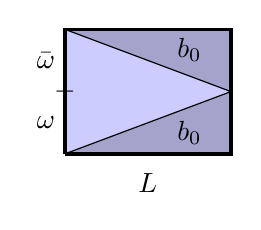
\begin{tikzpicture}[x=1.5em, y=1.5em, baseline=2.1em]
    \filldraw[very thick, fill=blue!20] (0,0)--(0,3)--(4,3)--(4,0)--(0,0);
    \draw (0,0)--(4,1.5)--(0,3);
    \filldraw[fill = black, opacity = 0.2] (0,0)--(4,1.5)--(0,3)--(4,3)--(4,0)--(0,0);
    \filldraw
    (0,.75) node[anchor=east]{$\omega$}
    (0,2.25) node[anchor=east]{$\bar\omega$}
    (0,1.5) node {$-$}
    (3,2.5) node {$b_0$}
    (3,0.5) node {$b_0$}
    (2,-0.7) node{$L$};
    \end{tikzpicture}
    \hspace{2cm}
    \(\displaystyle
    \begin{tikzcd}[column sep=huge]
    F_0\times
        
\begin{tikzpicture}[x=1em, y=1em, baseline=0.2em]
        \draw[very thick] (1,0)--(0,0)--(0,1)--(1,1);
        \end{tikzpicture}
    \arrow[r] \arrow[d,hook] & E \arrow[d,"p"] \\
    F_0\times
        
\begin{tikzpicture}[x=1em, y=1em, baseline=0.2em]
        \filldraw[very thick, fill=blue!20] (1,0)--(0,0)--(0,1)--(1,1)--(1,0);
        \end{tikzpicture}
    \arrow[ur,dashed,swap,"\bar L"] \arrow[r,swap,"L\circ\pr_{2,3}"] & B
    \end{tikzcd}\)
\end{center}